\begin{figure}[!htb]
\centering
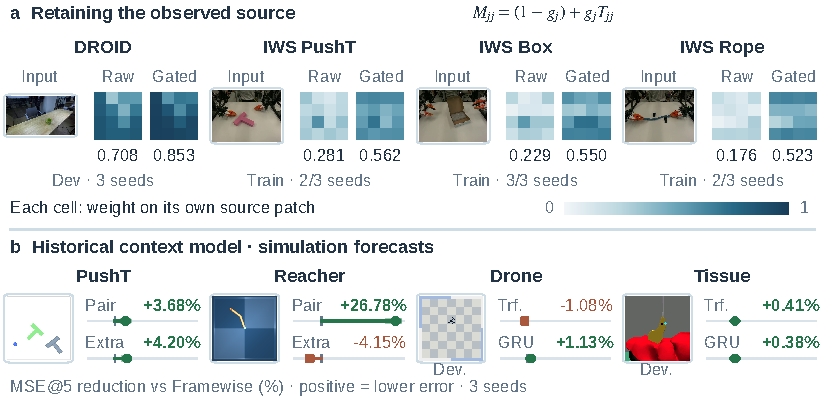
\includegraphics[width=\linewidth]{generated/editorial/decoder_evidence.pdf}
\caption[Spatial source retention and historical simulator forecasts.]{\textbf{Spatial source retention and historical simulator forecasts.}
\textbf{(a)} For ShiftWM's spatial decoder, each cell is one patch's own-source weight: the diagonal of raw mixing $T$ or effective mixing $M=I-D+DT$. All eight maps share a linear $[0,1]$ scale. Means below the maps average 16 patches and the displayed seeds, after forming $M$ per seed. Endpoints are DROID step 10 and IWS stored offset 59; case selection and training/development scope are specified above. These source weights precede the bounded correction. Their increase is a construction property, not an accuracy gain.
\textbf{(b)} The separate historical context model is compared with Framewise calibration using fixed-reference MSE@5. Pair/Extra denote held-out composition and the three-condition extrapolation aggregate; Trf./GRU denote both predictor architectures on drone/tissue development data. Positive values mean lower error. Dark markers and labels use the ratio of three-seed mean MSEs; pale dots are seedwise ratios. All stems share a $[-10,30]$ percent scale with a tick at zero; no confidence interval is implied. Simulator frames identify tasks, not scored examples.}
\label{fig:mixing-diagnostics}
\end{figure}
